\renewcommand{\thislecture}{4 }

%
% Cover page
%

\title[Neutrino Physics / Lecture \thislecture]
{
  {\huge \color{yellow} Neutrino Physics - Lecture \thislecture} \\
  {\it 3-Flavour Neutrino Oscillations:\\ Unresolved Questions, Future Prospects}\\
}

\author[C.Andreopoulos] {
  Professor Costas Andreopoulos\inst{1,2}
}
\institute[Liverpool/STFC-RAL] {
   \inst{1} University of Liverpool,
   \inst{2} STFC Rutherford Appleton Laboratory\\
   \vspace{0.5cm}
   {\it {\color{magenta} A post-graduate student lecture course}}\\
   \vspace{0.2cm}
}
\date{\today}

\titlegraphic{
  
\includegraphics[height=25px]{./images/logo/liverpool.png}
  \hspace{3px}
  
\includegraphics[height=30px]{./images/logo/ral.png}
}

	



\begin{frame}[plain]
  \titlepage
\end{frame}

%
% Outline
%

\begin{frame}{Outline for Lecture \thislecture}

\begin{itemize}
  \item Current picture
  \item Unresolved questions
  \item Near-future LBL sensitivity (T2K and NOvA)
  \item The future
  \begin{itemize}
    \item LBL reactor experiments: JUNO, RENO-50
    \item Telescopes: IceCube/PINGU, ORCA/ARCA
    \item LBL accelerator experiments: DUNE, HK
  \end{itemize}
\end{itemize}

\end{frame}

%
%
%

\begin{frame}{3-Flavour Oscillations: The current picture}

\begin{columns}[T]
  \begin{column}{0.55\textwidth}
    \begin{center}
     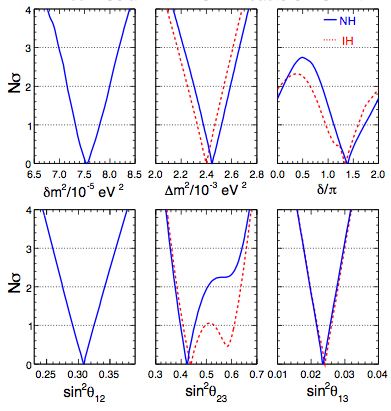
\includegraphics[width=0.98\textwidth]{./images/3nu/global_fits/fl-chisq.png}\\
    \end{center}
  \end{column}
  \begin{column}{0.45\textwidth}
    \begin{center}
     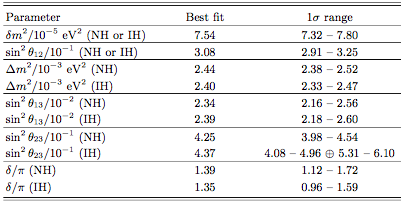
\includegraphics[width=0.98\textwidth]{./images/3nu/global_fits/fl-table.png}\\
    \end{center}
    {\tiny
      F.Capozzi, G.L.Fogli, E.Lisi, A.Marrone, D.Montanino, and A.Palazzo, Status of three-neutrino oscillation
      parameters, circa 2013, arXiv:1312.2878\\
    }
  \end{column}
\end{columns}
\end{frame}


\begin{frame}{Unresolved questions}

\begin{columns}[T]
  \begin{column}{0.70\textwidth}
     Next {\em deep questions} to address with oscillation experiments:\\
     \vspace{0.4cm}
     \begin{itemize}
       \item What is the mass hierarchy?
       \vspace{0.3cm}
       \item Is $\theta_{23}$ maximal?
         \begin{itemize}
           \item If not, what is the $\theta_{23}$ octant?
         \end{itemize}
       \vspace{0.3cm}
       \item {\bf Do neutrinos violate CP invariance?}
       \vspace{0.3cm}
       \item {\bf Is the PMNS matrix unitary?}
     \end{itemize}
  \end{column}
  \begin{column}{0.05\textwidth}
  \end{column}
  \begin{column}{0.25\textwidth}
    \begin{block}{}
     {\color{magenta}
        {\tt \small
         `A deep question is one where either a yes
          or no answer is interesting.'\\}
          \vspace{0.3cm}
          N.Bohr
     }
    \end{block}
  \end{column}
\end{columns}
\end{frame}


%
% Near future sensitivity
%

\begin{frame}{Near-Future LBL Accelerator Expt Sensitivity (T2K)}

{\tiny T2K Future Sensitivity results from T2K report to 2013 J-PARC PAC. Publication in progress.}
\begin{columns}[T]
  \begin{column}{0.63\textwidth}
  {
    \begin{center}
     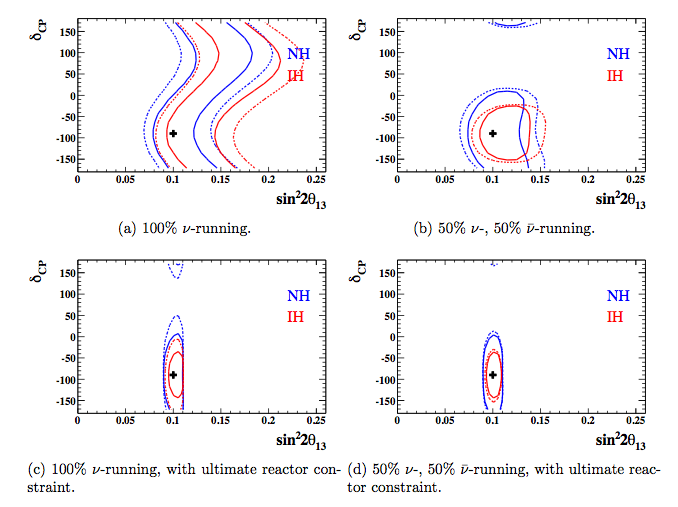
\includegraphics[width=0.98\textwidth]{./images/3nu/accelerator/future_sensitivity/t2k/deltacp_sensitivity_2x2cases_minuspi2.png}\\
    \end{center}
  }
  \end{column}
  \begin{column}{0.36\textwidth}
    \vspace{0.3cm}
    {\scriptsize
     \begin{itemize}
       \item Difference in $\delta_{CP}$ sensitivity with $\nu$-enhanced and $\bar{\nu}$-enhanced beam running.
       \vspace{0.1cm}
       \item Improved sensitivity with a combination of $\nu$ and $\bar{\nu}$ data.
       \vspace{0.1cm}
       \item {\bf $\sim$90\% C.L. measurement for certain true values of $\delta_{CP}$.}
       \vspace{0.1cm}
       \item Similar $\delta_{CP}$ constraint with and without the reactor data:
             {\bf Could start over-constraining the PMNS framework.}
     \end{itemize}
    }
  \end{column}
\end{columns}
\noindent\rule{2cm}{0.4pt}\\
{\tiny
  {\bf 90\% C.L. intervals for true NH and true $\delta_{CP}=-\pi/2$},
   $sin^{2}2{\theta}_{13}$=0.1, $sin^{2}{\theta}_{23}$=0.5, ${\Delta}m^{2}_{32}$=2.4$\times10^{-3}$ $eV^{2}/c^{4}$.\\
   Blue: Correct hierachy, Red: Incorrect hierarchy -
   Solid: Statistical errors only, Dashed: With 2012 systematics.\\
   Assumed exposure: $7.8\times10^{21}$ protons on target.
   Assumed ultimate reactor constraint: $\delta(sin^{2}2{\theta}_{13})$=0.005.\\
   Fully correlated $\nu$ and $\bar{\nu}$ systematic errors.\\
}
\end{frame}


\begin{frame}{Near-Future LBL Accelerator Expt Sensitivity (T2K)}

%\begin{center}
 {\small \centering
   Sensitivity to $\delta_{CP}$ depends strongly on its true value.\\
   Plots below show the calculated {\bf $\Delta\chi^{2}$ for the $sin({\delta}_{CP})$ = 0 hypothesis}
   for different values of $\delta_{CP}$ and $\theta_{23}$.\\
 }
%\end{center}

\begin{columns}[T]
  \begin{column}{0.48\textwidth}
  {
    \begin{center}
      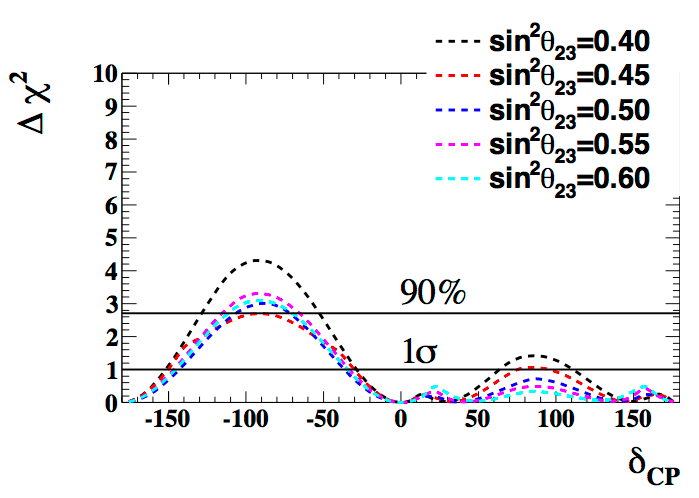
\includegraphics[width=0.99\textwidth,height=0.45\textheight]{./images/3nu/accelerator/future_sensitivity/t2k/exclude_sindelta0_50nu50nubar_nh_selected_theta23.png}\\
    \end{center}
  }
  \end{column}
  \begin{column}{0.52\textwidth}
    \begin{center}
      \vspace{0.3cm}
      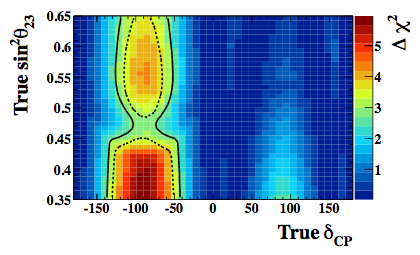
\includegraphics[width=0.99\textwidth,height=0.45\textheight]{./images/3nu/accelerator/future_sensitivity/t2k/exclude_sindelta0_50nu50nubar_nh.png}\\
    \end{center}
  \end{column}
\end{columns}

\noindent\rule{2cm}{0.4pt}\\
{\tiny
 True: NH, $sin^{2}2{\theta}_{13}$=0.1, ${\Delta}m^{2}_{32}$=2.4$\times10^{-3}$ $eV^{2}/c^{4}$.\\
 Solid: Statistical errors only, Dashed: With 2012 systematics.\\
 Assumed exposure: $7.8\times10^{21}$ protons on target.
 Assumed ultimate reactor constraint: $\delta(sin^{2}2{\theta}_{13})$=0.005.\\
 Assumed a $\nu$:$\bar{\nu}$ = 1:1 running scenario with fully correlated systematic errors.\\
}
\end{frame}



\begin{frame}{Near-Future LBL Accelerator Expt Sensitivity (T2K)}

\begin{columns}[T]
  \begin{column}{0.60\textwidth}
  {
    \begin{center}
     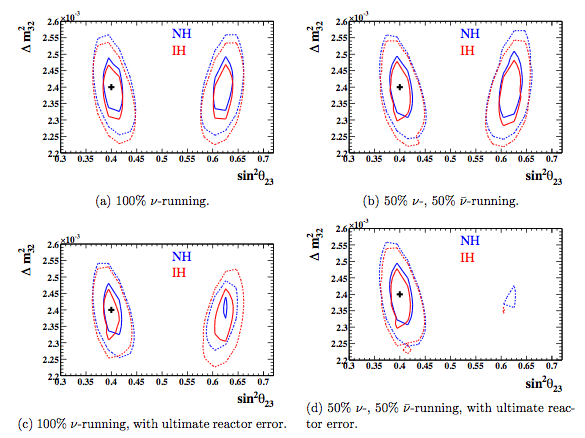
\includegraphics[width=0.99\textwidth]{./images/3nu/accelerator/future_sensitivity/t2k/disapp_dm_vs_sinsq23_90cl_2octants_2x2.png}\\
    \end{center}
    \vspace{0.2cm}
  }
  \end{column}
  \begin{column}{0.40\textwidth}
    \vspace{0.4cm}
    {\scriptsize
     \begin{itemize}
        \item Added power from combining $\nu$ and $\bar{\nu}$ data
              compensates for loss of statistics in  $\bar{\nu}$-enhanced beam mode.
              There is no effect on the disappearance measurement using T2K data alone.
        \vspace{0.2cm}
        \item Combination of T2K $\nu$ and $\bar{\nu}$ data and reactor data
              could allow us to resolve the $\theta_{23}$ octant.
     \end{itemize}
    }
  \end{column}
\end{columns}
\noindent\rule{2cm}{0.4pt}\\
{\tiny
  {\bf 90\% C.L. intervals for true NH and true ${\Delta}m^{2}_{32}$=2.4$\times10^{-3}$ $eV^{2}/c^{4}$, $sin^{2}{\theta}_{23}$=0.4},
      ${\delta}_{CP}=0$ and $sin^{2}2{\theta}_{13}$=0.1.\\
      Blue: Correct hierachy, Red: Incorrect hierarchy -
      Solid: Statistical errors only, Dashed: With 2012 systematics.\\
      Assumed exposure: $7.8\times10^{21}$ protons on target.
      Assumed ultimate reactor constraint: $\delta(sin^{2}2{\theta}_{13})$=0.005.\\
      Fully correlated $\nu$ and $\bar{\nu}$ systematic errors.\\
}
\end{frame}



\begin{frame}{Near-Future LBL Accelerator Expt Sensitivity (T2K)}

\begin{columns}[T]
  \begin{column}{0.66\textwidth}
    \begin{center}
      {\bf \scriptsize
         Values of $sin^{2}{\theta}_{23}$ for which maximal mixing and the wrong octant
         can be rejected at the stated C.L.\\
      }
      \vspace{0.1cm}
      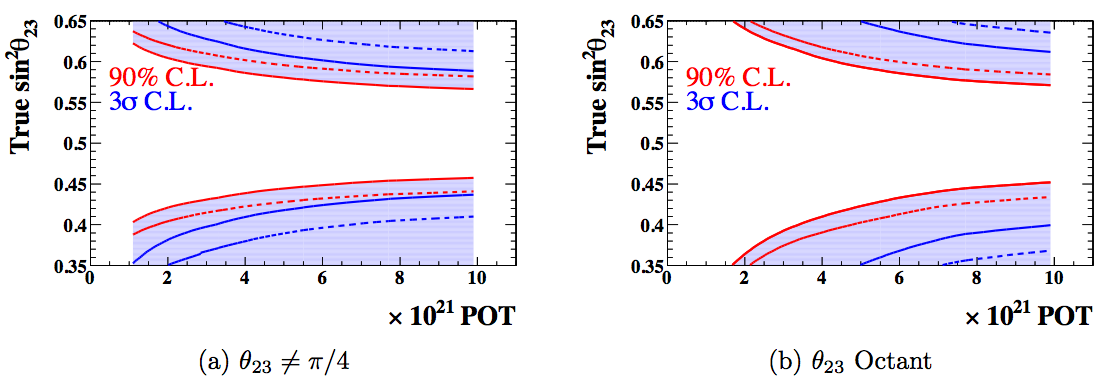
\includegraphics[width=0.94\textwidth]{./images/3nu/accelerator/future_sensitivity/t2k/max23mix_octant_resulution.png}\\
      {\scriptsize
         $\theta_{23}$ octant could be determined at 90\% C.L. if $|\theta_{23}-45^{o}| > 4^{o}$.
      }
    \end{center}
    \noindent\rule{2cm}{0.4pt}\\
    {\tiny
      {\bf 2 left plots:}\\
      True: NH, ${\delta}_{CP}=0$, $sin^{2}2{\theta}_{13}$=0.1, ${\Delta}m^{2}_{32}$=2.4$\times10^{-3}$ $eV^{2}/c^{4}$.\\
      Solid: Statistical errors only, Dashed: With 2012 systematics.\\
      \vspace{0.1cm}
      {\bf 2 right plots:}\\
      True: NH, ${\delta}_{CP}=0$, $sin^{2}2{\theta}_{13}$=0.1, $sin^{2}{\theta}_{23}$=0.5, ${\Delta}m^{2}_{32}$=2.4$\times10^{-3}$ $eV^{2}/c^{4}$.\\
      Solid: Statistical errors only, Dashed: With projected systematics.\\
      \vspace{0.1cm}
      {\bf All plots:}\\
      Assumed a $\nu$:$\bar{\nu}$ = 1:1 running scenario
      with fully correlated systematic errors.\\
      Assumed ultimate reactor constraint: $\delta(sin^{2}2{\theta}_{13})$=0.005.\\
    }
  \end{column}
  \begin{column}{0.33\textwidth}
    \begin{center}
      {\bf \scriptsize
         1$\sigma$ err for $sin^{2}{\theta}_{23}$ and ${\Delta}m^{2}_{32}$ as function of T2K exposure.\\
      }
      \vspace{0.1cm}
      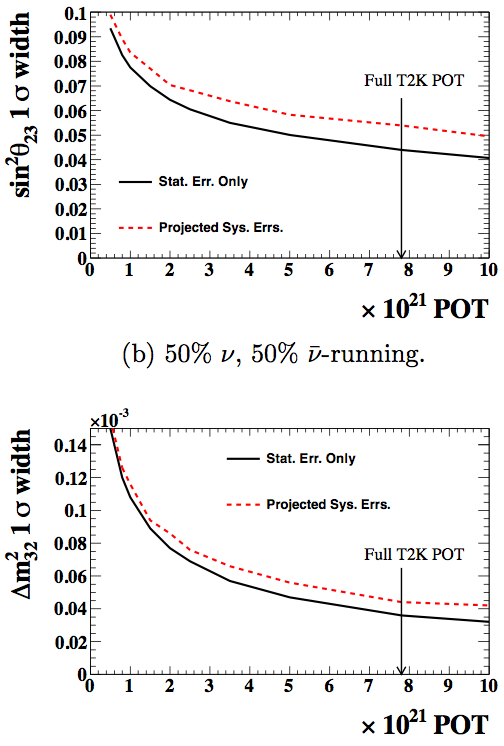
\includegraphics[width=0.90\textwidth]{./images/3nu/accelerator/future_sensitivity/t2k/disapp_dm_theta23_sigma.png}\\
      {\scriptsize
         ${\delta}(sin^2\theta_{23})$ $\simeq$ 0.045 (2.6$^{o}$)\\
         ${\delta}({\Delta}m^{2}_{32})$ $\simeq$ 4$\times10^{-5}$ $eV^{2}/c^{4}$\\
      }
    \end{center}
  \end{column}
\end{columns}
\end{frame}



\begin{frame}{Near-Future LBL Accelerator Expt Sensitivity (NOvA)}

NOvA, which is quite complementary to T2K has also started taking data quite recently.\\
\begin{center}
  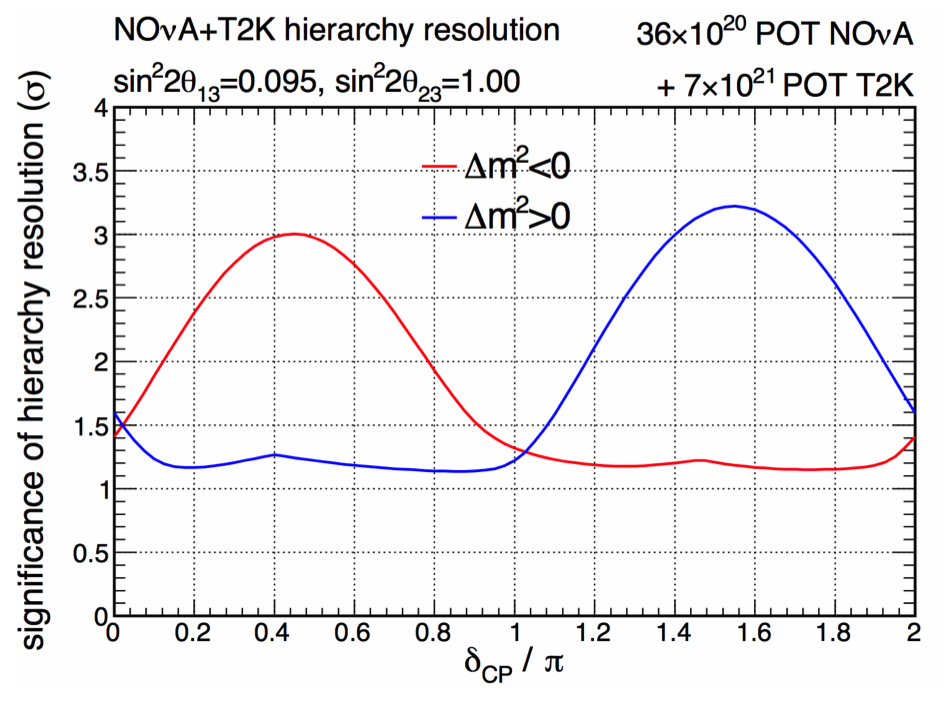
\includegraphics[width=0.60\textwidth]{./images/3nu/accelerator//future_sensitivity/nova/nova-hierarchy.png}\\
\end{center}
{\scriptsize \color{blue}[Andrew Norman, Neutrino 2014 conference, Boston]}

\end{frame}

%
% Conslusions for sensitivity by 2020
%


\begin{frame}{LBL Accelerator Oscillation in the next decade}

{\scriptsize
{\bf T2K+NOvA could establish that $sin(\delta_{CP})\ne0$,
the MH and $\theta_{23}$ octant at up to ~3$\sigma$.}\\
\vspace{0.2cm}
{\color{red}... if we are lucky with the true values of oscillation parameters.}\\
\vspace{0.4cm}

Note:\\
The actual observed significance can be \underline{much better} than the projected sensitivity
\begin{itemize}
  \item For the latest T2K $\nu_{e}$ appearance result, the observed
        significance was 7.3$\sigma$ whereas the projected sensitivity was 5.3$\sigma$.\\
\end{itemize}
\vspace{0.2cm}
{\color{red}... of course, actual observed significance can also be worst than the projected sensitivity.}\\
\vspace{0.5cm}

{\bf A new generation of experiments is needed to extend our sensitivity} to:
\begin{itemize}
 \item neutrino CP violation
 \item neutrino mass hierarchy
 \item deviations from the 3-flavour paradigm
\end{itemize}
The level of investment necessary to realize a next generation experiment
requires that we design experiments with proven and {\bf \underline{compelling sensitivity}}.
}

\end{frame}



%
%
% The future
%
%


\begin{frame}{Future long-baseline reactor experiments}

{\small
 {\bf LBL reactor experiment with a very large liquid scintillator detector:}\\
 Can observe simultaneously the wiggles from oscillations at the solar and atmospheric
 squared-mass splittings.\\
}
\begin{columns}[T]
  \begin{column}{0.55\textwidth}
    \centering
     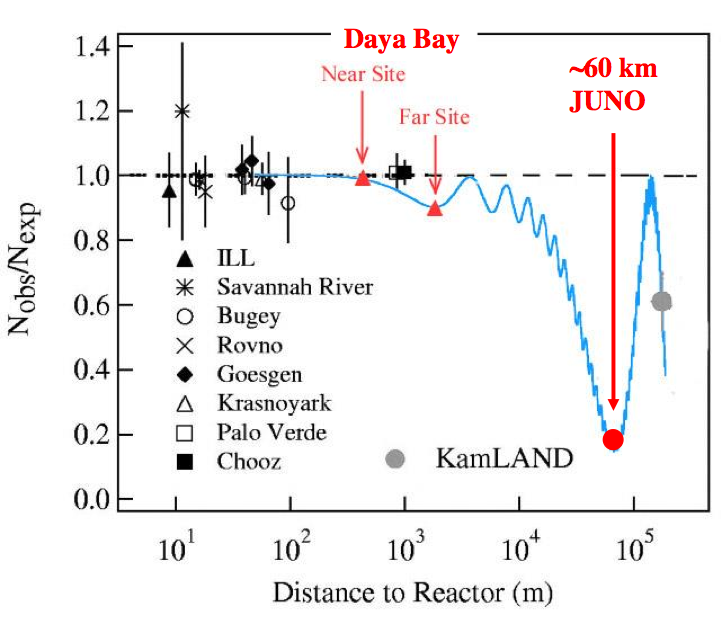
\includegraphics[width=0.98\textwidth]{./images/3nu/reactor/juno_deficit_vs_distance.png}\\
  \end{column}
  \begin{column}{0.45\textwidth}
  {\scriptsize
      {\bf \color{red}Primary goals:}\\
      \begin{itemize}
       {\color{red}
        \item Determination of the mass hierarchy
        \item Precision measurements of ${\Delta}m^{2}_{31}$, ${\Delta}m^{2}_{21}$, $\theta_{12}$
       }
      \end{itemize}
      Such a large detector would also develop a rich physics programme:\\
      \begin{itemize}
        \item Supernova neutrinos
        \item Solar neutrinos
        \item Atmospehric neutrinos
        \item Geo-neutrinos
        \item Sterile neutrinos
      \end{itemize}
  }
  \end{column}
\end{columns}
\end{frame}



\begin{frame}{Future LBL reactor experiments: JUNO \& RENO-50}

{\small
JUNO (Jiangmen Underground Neutrino Observatory) in China: A 20 kt liquid scintillator detector
observing $\bar{\nu}_{e}$ from 2 reactor complexes (Taishan and Yangjiang) with an average baseline
of 52.5 km (0.25 km RMS). The combined power of the power plants is 35.8 GW
{\scriptsize \color{blue}[Phys. Rev. D 88, 013008 (2013)]}.
}
\begin{columns}[T]
  \begin{column}{0.55\textwidth}
    \centering
     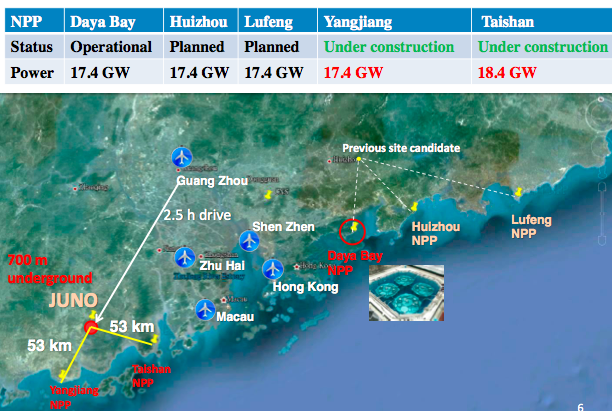
\includegraphics[width=0.98\textwidth]{./images/3nu/reactor/juno_location.png}\\
  \end{column}
  \begin{column}{0.45\textwidth}
     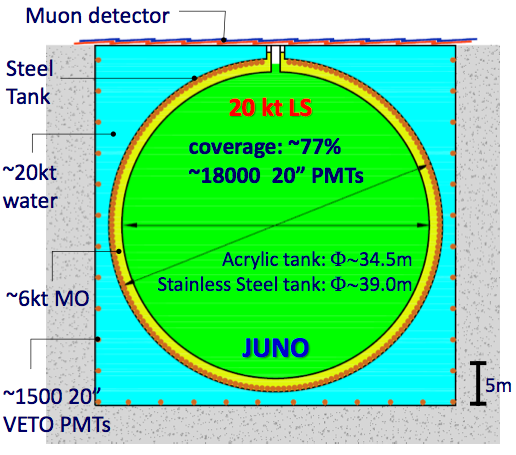
\includegraphics[width=0.98\textwidth]{./images/3nu/reactor/juno_schematic.png}\\
  \end{column}
\end{columns}
A similar experiment (RENO-50) is proposed in S.Korea.
\end{frame}



\begin{frame}{JUNO mass hierarchy sensitivity}

Energy resolution would be critical for the MH determination.
\begin{columns}[T]
  \begin{column}{0.55\textwidth}
    \centering
     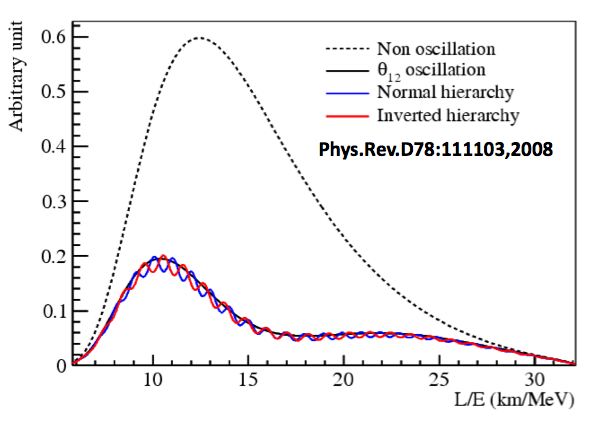
\includegraphics[width=0.98\textwidth]{./images/3nu/reactor/juno_wiggles.png}\\
%    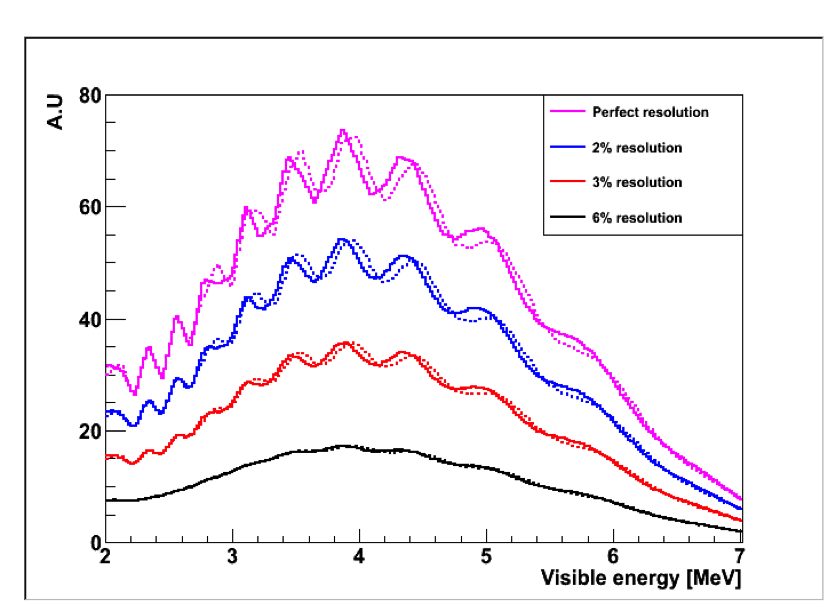
\includegraphics[width=0.60\textwidth]{./images/3nu/reactor/reno50_wiggles_disappear.png}\\
%    {\tiny Bottom plot by J.Park for RENO-50}
  \end{column}
  \begin{column}{0.45\textwidth}
     {\color{red}JUNO is aiming for 3\%/$\sqrt{E}$ energy resolution}\\
     \vspace{0.4cm}
     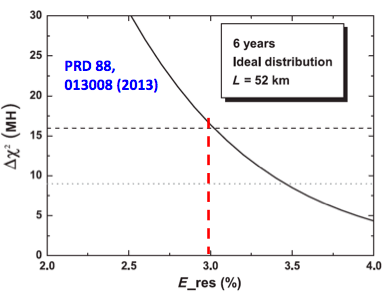
\includegraphics[width=0.98\textwidth]{./images/3nu/reactor/juno_MHsign_vs_Eresolution.png}\\
  \end{column}
\end{columns}
\end{frame}


\begin{frame}{Atmospherics: PINGU}
\begin{columns}
  \begin{column}{0.50\textwidth}
   \centering
   {\scriptsize
    PINGU (Precision IceCube Next Generation Upgrade) {\color{blue}[arXiv:1401.2046]}:\\
    In-fill array for IceCube\\
    (40 strings, ~20m spacing, 3-5m DOM spacing)\\
   }
   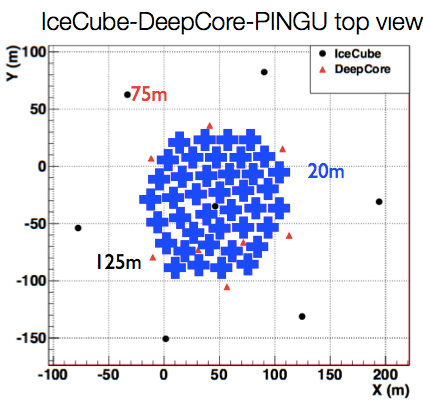
\includegraphics[width=0.65\textwidth]{./images/3nu/atmo/pingu_topview.png}\\
   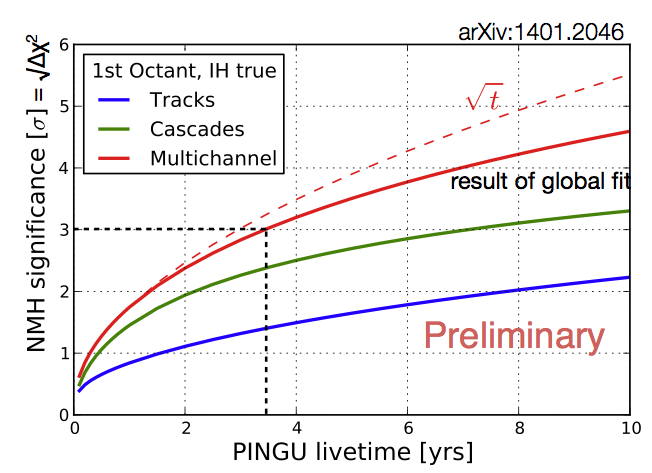
\includegraphics[width=0.65\textwidth]{./images/3nu/atmo/pingu_sensitivity.png}\\
  \end{column}
  \begin{column}{0.50\textwidth}
   \centering
    {\scriptsize $\sim$20\% difference in $\pbar{\nu}_{\mu}$ due to matter effects}
    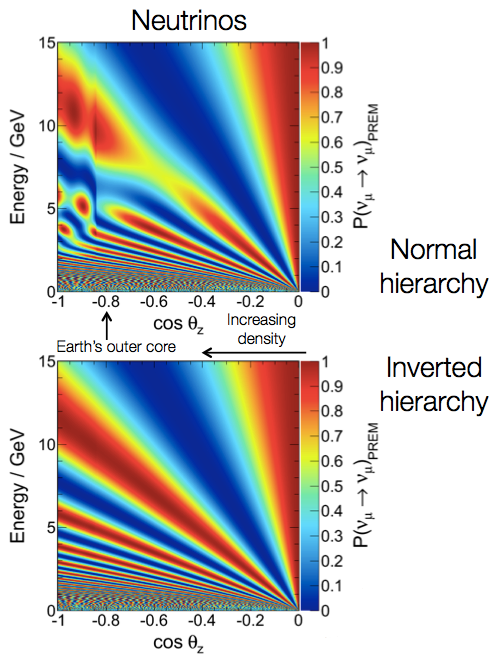
\includegraphics[width=0.85\textwidth]{./images/3nu/atmo/pingu_oscillogram.png}\\
    {\scriptsize {\color{blue}[Grant, Neutrino 2014, Boston]}}\\
  \end{column}
\end{columns}
\end{frame}



\begin{frame}{Main approaches for future LBL accelerator experiments}

\begin{columns}[T]
  \begin{column}{0.48\textwidth}
      {\scriptsize
        {\bf $\sim$40kt LAr detector in wide-band beam}\\
        \begin{itemize}
          \item Bubble-chamber-like imaging but not well known technology
          \item Relatively dense material $\rightarrow$ secondary re-interactions complicating event topologies
          \item Technology allows reconstruction of multi-particle event topologies and calorimetric energy reconstruction.
          \item Can work in high-E$_{\nu}$ wide-band beams
          \item Wide band and good energy resolution $\rightarrow$ rich spectral information
                (e.g. redundancy in $\delta_{CP}$ measurements, discrimination between $\delta_{CP}$=0 or $\pi$,
                increased sensitivity to exotic physics scenarios).
         \item High E$_{\nu}$ $\rightarrow$ Very long baseline
         \item Very long baseline $\rightarrow$ Matter effects
         \item Matter effects $\rightarrow$ Sensitivity to MH (as well as $\delta_{CP}$) with beam neutrinos
        \end{itemize}
      }
  \end{column}
  \begin{column}{0.52\textwidth}
      {\scriptsize
        {\bf $\sim$200kt water Ckv detector in narrow-band beam}\\
        \begin{itemize}
         \item Very well-known detector technology.
         \item Excellent detection capabilities for charged leptons but largely blind to the details of the hadronic system.
         \item Golden oscillation analysis samples are CCQE-enhanced 1-ring e-like and 1-ring $\mu$-like samples.
         \item Works best at relatively low-energy narrow-band beams
         \item Narrow band  $\rightarrow$ limited spectral information
         \item Low energy $\rightarrow$ Not very long baseline
         \item Not very long baseline  $\rightarrow$ No matter effects
         \item No matter effects  $\rightarrow$ No MH sensitivity with beam $\nu$'s.
         \item Excellent $\delta_{CP}$ sensitivity comparing $\nu$/$\bar{\nu}$ running if MH is known
         \item But MH has to come from somewhere else (or atmospherics, $\sim$3$\sigma$ in 10 yrs)
        \end{itemize}
      }
  \end{column}
\end{columns}
\end{frame}


\begin{frame}{The DUNE experiment}
\begin{columns}
  \begin{column}{0.50\textwidth}
   \begin{itemize}
   {\scriptsize
     \item Very long-baseline (Fermilab to SURF, 1300km) experiment in a wide-band beam
     \item Upgraded beam power (Fermilab PIP-II): 60-120 GeV protons
           1.2 MW at startup (2.3 MW upgrade capability)
     \item Deep underground (SURF, 4850 ft)
     \item $>$40kt fiducial ($\sim$70kt total) liquid Argon TPC far detector.
%          \begin{itemize}
%          {\scriptsize
%             \item
             (baseline: single phase, based on ICARUS design,
             but with industrial cryostat and cold electronics)
%          }
%          \end{itemize}
     \item Highly capable near detectors $\sim$ 450 m from target
     \item Very rich physics program:
        {\scriptsize
            \item Neutrino oscillations with accelerator, atmospheric and solar neutrinos
            \item Proton decay searches
            \item Neutrino astrophysics (supernova bursts, relic neutrinos, dark matter)
         }

   }
   \end{itemize}
  \end{column}
  \begin{column}{0.50\textwidth}
    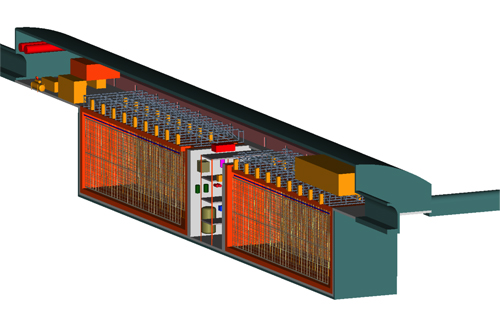
\includegraphics[width=0.98\textwidth]{./images/3nu/accelerator/lbne_doublecryo_schematic.jpg}\\
    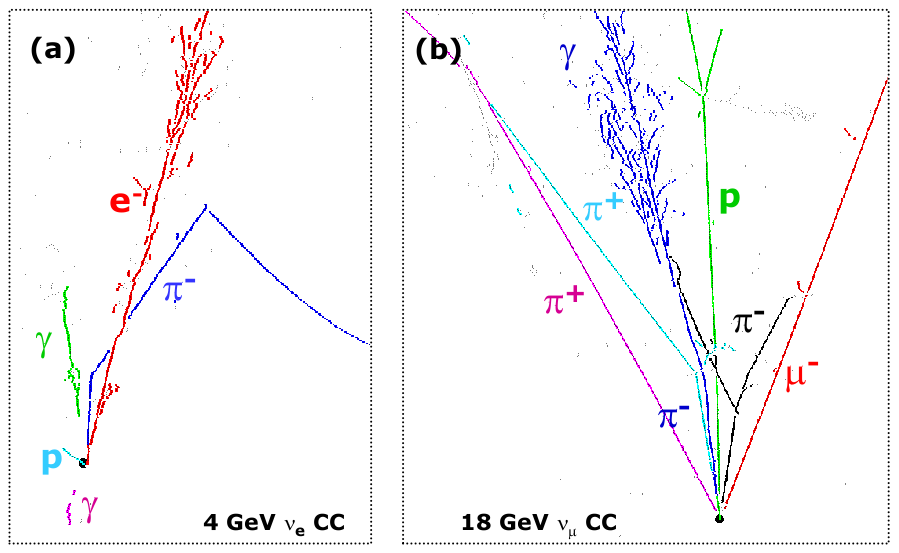
\includegraphics[width=0.98\textwidth]{./images/3nu/accelerator/lar_display.png}\\
  \end{column}
\end{columns}
\end{frame}


\begin{frame}{DUNE LArTPC}

\begin{center}
  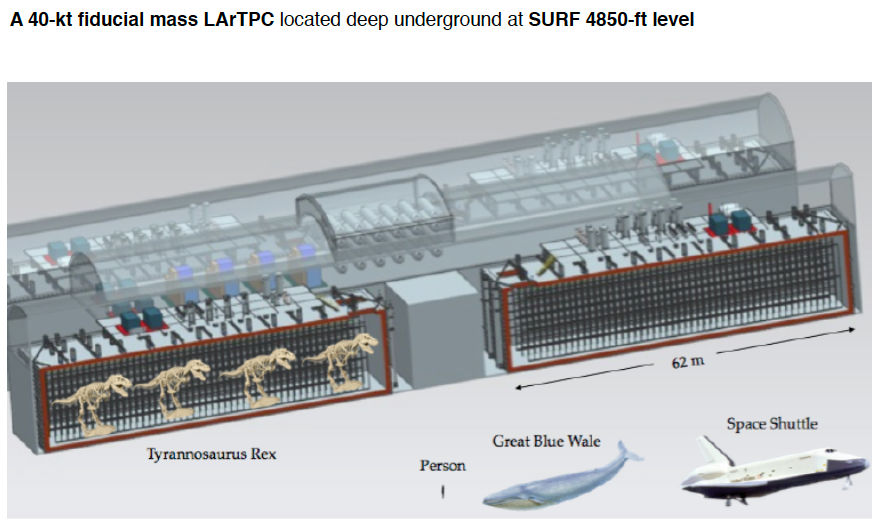
\includegraphics[width=0.98\textwidth]{./images/3nu/future/lartpc_1}\\
\end{center}

\end{frame}

\begin{frame}{DUNE LArTPC}

\begin{center}
  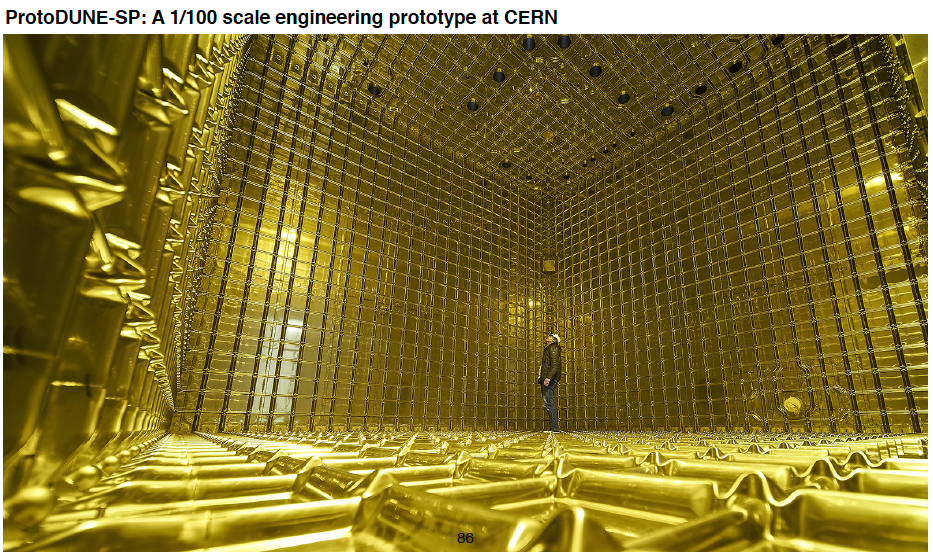
\includegraphics[width=0.98\textwidth]{./images/3nu/future/lartpc_2}\\
\end{center}

\end{frame}

\begin{frame}{LArTPCs: How do they work?}

\begin{center}
  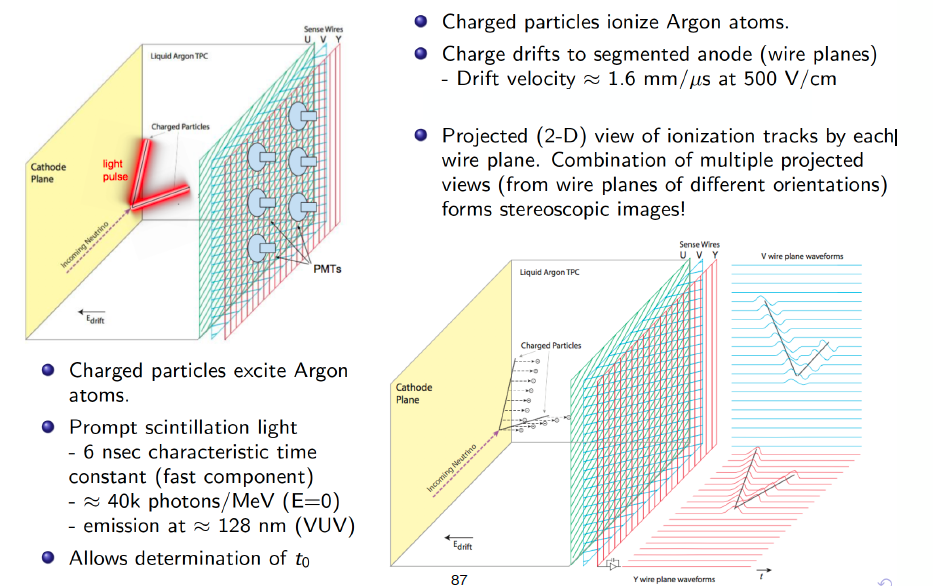
\includegraphics[width=0.98\textwidth]{./images/3nu/future/lartpc_3}\\
\end{center}

\end{frame}

\begin{frame}{LArTPCs for neutrino physics}

\begin{center}
  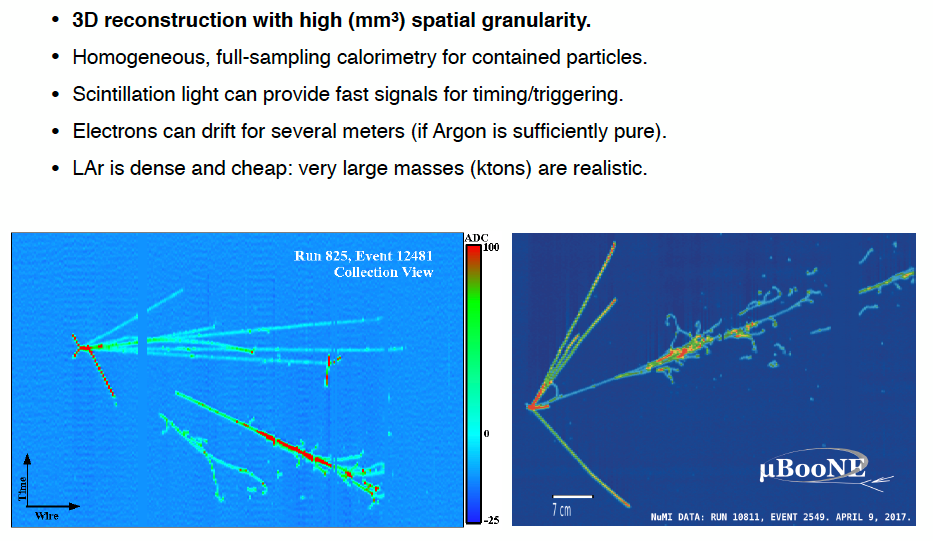
\includegraphics[width=0.98\textwidth]{./images/3nu/future/lartpc_4}\\
\end{center}

\end{frame}

\begin{frame}{LArTPCs: Electronic bubble chambers}

\begin{center}
  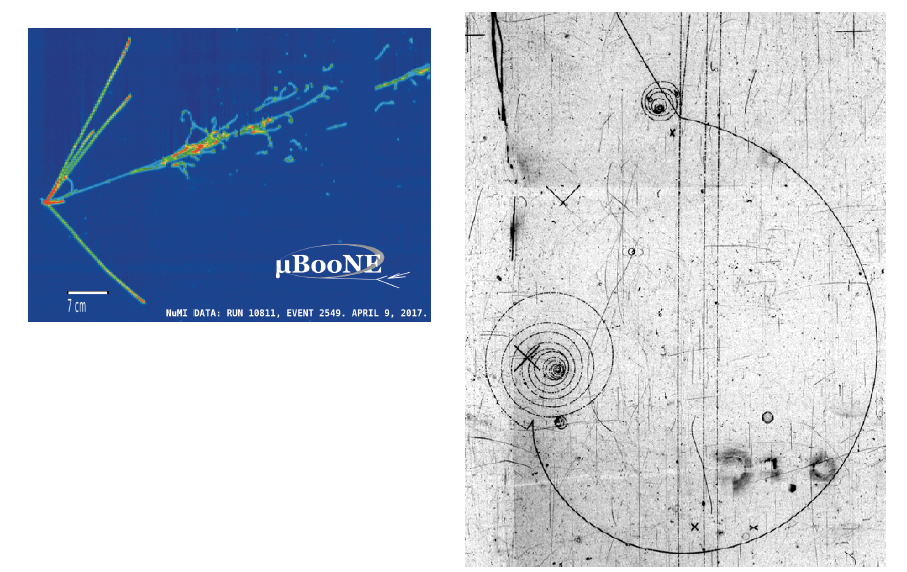
\includegraphics[width=0.98\textwidth]{./images/3nu/future/lartpc_5}\\
\end{center}

\end{frame}


\begin{frame}{DUNE physics potential}

  \begin{center}
    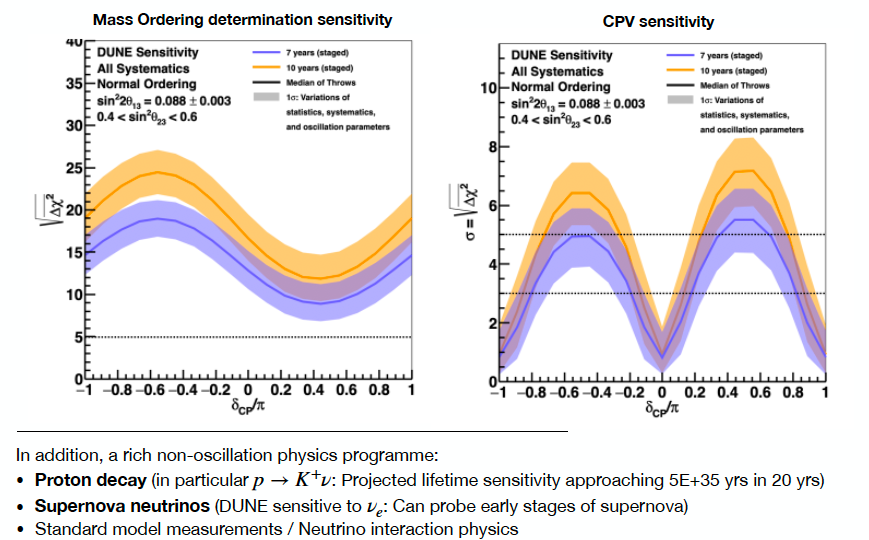
\includegraphics[width=0.98\textwidth]{./images/3nu/future/dune_phys_potential_page}\\
  \end{center}

% 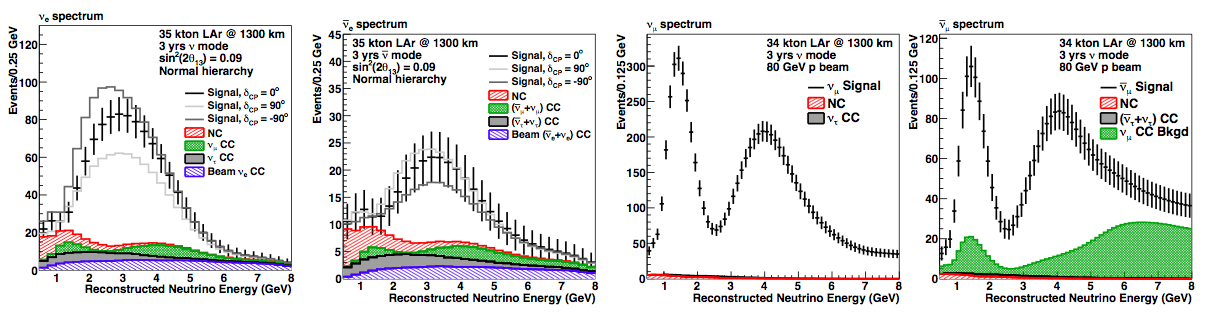
\includegraphics[width=0.98\textwidth]{./images/3nu/accelerator/lbne_spectra.png}\\
% \begin{columns}
%   \begin{column}{0.35\textwidth}
%     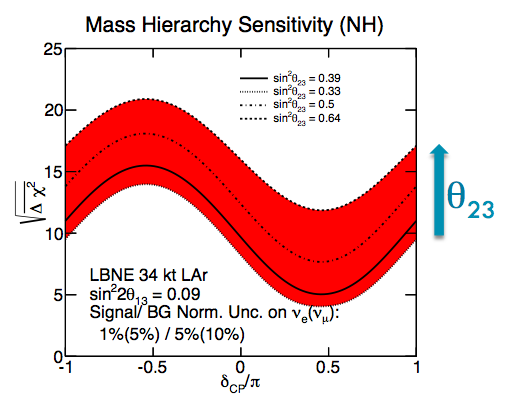
\includegraphics[width=0.98\textwidth,height=0.40\textheight]{./images/3nu/accelerator/lbne_mh_sensitivity.png}\\
%   \end{column}
%   \begin{column}{0.35\textwidth}
%     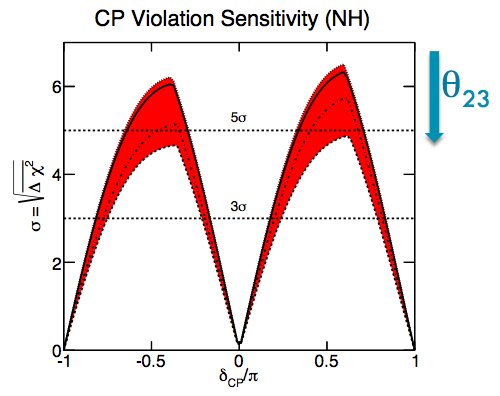
\includegraphics[width=0.98\textwidth,height=0.40\textheight]{./images/3nu/accelerator/lbne_sindcp0_sensitivity.png}\\
%   \end{column}
%   \begin{column}{0.31\textwidth}
%     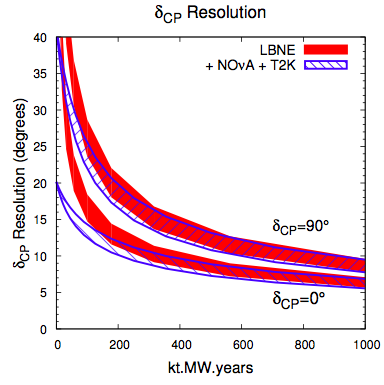
\includegraphics[width=0.98\textwidth,height=0.40\textheight]{./images/3nu/accelerator/lbne_dcp_resolution.png}\\
%   \end{column}
% \end{columns}
%
% {\scriptsize
%   {\centering \color{blue}[Worcester, NOW 2014 conference]}\\
% }
\end{frame}



\begin{frame}{The Hyper-Kamiokande experiment}

{\scriptsize A natural extension of the T2K programme
(Tokai to Kamioka, in J-PARC narrow band beam)}\\

\vspace{0.3cm}

\begin{columns}[t]
  \begin{column}{0.49\textwidth}
    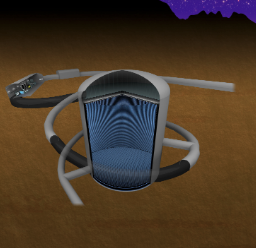
\includegraphics[width=0.98\textwidth]{./images/3nu/accelerator/hyperk_schematic_2021a}\\
  \end{column}
  \begin{column}{0.50\textwidth}
    \vspace{-3.7cm}
    \begin{itemize}
    {\scriptsize
       \item 258 kton water Cherenkov detector
       \item 187 kton fiducial ($>$8 $\times$ Super-K)
       \item Improved PMTs, $\times$2 photo detection efficiency
       \item New Intermediate Water Cherenkov Detector (IWCD)
       \item Upgraded Near Detector (ND280)
       \item J-PARC beam upgraded to 1.3 MW
       \item Operations in 2027\\
    }
    \end{itemize}
  \end{column}
\end{columns}
\end{frame}


\begin{frame}{Hyper-Kamiokande physics sensitivity}

Excellent CPV sensitivity and measurement resolution.\\
\vspace{0.2cm}
\begin{columns}[t]
    \begin{column}{0.50\textwidth}
      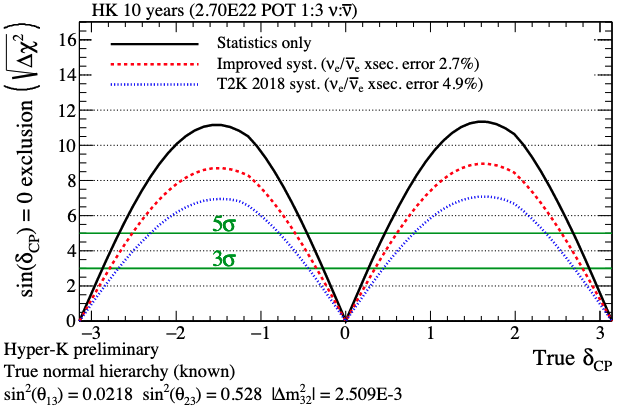
\includegraphics[width=0.98\textwidth]{./images/3nu/accelerator/hyperk_new_cpv_2021_a}\\
    \end{column}
    \begin{column}{0.50\textwidth}
      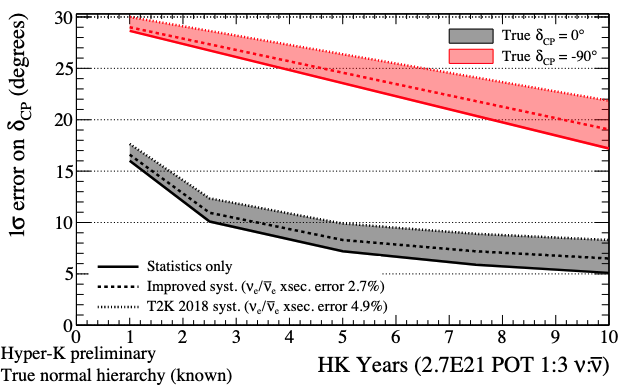
\includegraphics[width=0.98\textwidth]{./images/3nu/accelerator/hyperk_new_cpv_2021_b}\\
    \end{column}
\end{columns}

\noindent\rule{2cm}{0.4pt}\\
{\scriptsize
Similarly with DUNE, HyperK has rich non-oscillation physics potential.
}

\end{frame}

%
%
%

% \begin{frame}{What to read}
%
% {\color{magenta} Add in next revision}
%
% \end{frame}
